\chapter{Sampling on Hadoop} % (fold)
\label{cha:sample}

\section{Motivation for sampling}

One relevant aspect in Big Data environment is to work with vast amounts of data,
such fact is the main barrier to find a good configuration of one job. The bacteriological
algorithm is a good option to create new configurations, but these configurations
must be tested in order to select what is the best for the job in question at the
moment. Other relevant issue in this type of environment is your volatility, caused
by constant variation of the data, i.e. insertion or remotion of data constantly.
Also due processing the large amounts of data the power computing depends of hundreds
or even thousands of machines and it may fail, this fails characterize changes on
the environment what can invalidate the current configuration for the job.

Therefore, there is one cycle on the Big Data environment that is to select one
configuration for a given job and execute the job, and again chosen one configuration
and execute the job etc. Such cycle must repeat on the environment due your feature
of high volatility.

One issue stay in the air: {\it how must we test and select the job configurations
generated by bacteriological algorithm?} One possible answer is to run the job with
sample data, because the job wouldn't run on all data stored what would spend too
much time and also would be impracticable due larger number of intermediate
configurations generated by the algorithm.

\section{Challenge for sampling in Big Data environment}

On Big Data environment there are several aspects involving computing and storage
distributed. For data sample the aspects involving storage distributed are more
relevant. In this context, without doubt, the data volume is the main issue because
the data sampling must be done distributed too, otherwise one machine couldn't bear
all data storage in the cluster then make the data sampling. Also the data sampling
resultant must be storage distributed in the cluster, because even being a sample
the result can be big and a single machine couldn't bear too.

So the sampling must be done distributed and it must be done without intrusion
in the Hadoop, because any change done inside of the framework can propagate collateral
effects due its complexity. Further more to run test regression is a very costly
activity~\cite{hadoopUnit} and to create unit test cases for the new changes spend
much time.

One way to sample data on Hadoop is to utilize its benefits, i.e. to benefit of
its structure of storage and computing distributed. We can build one MapReduce
program to sample data and so we will be benefiting of its advantages as framework
to distributed computing.

One of the most used data sample techniques is {\bf Random Sampling} that consists
basically in select a pre-determined amount or percentage of data randomly~\cite{randomsampling}.
In the literature there are several others techniques such as {\bf Stratified Random Sampling},
this techniques splits the data in strata in which each element has the same chance
of being selected~\cite{randomsampling}. Another thechnique is {\bf Systematic Sampling}
that chooses randomly the first element and then till the k-esimo element in sequence
is selected~\cite{systematicsampling}.

In the context of big data there are some implementations of data sample. One example
is the {\bf MonetDB} which is column-oriented database management system and was
designed to hold data in main-memory and processes large-scale data distributed~\cite{monetDB},
this database support data sample and use the {\it Algorithm A} that is based in
random sample method~\cite{vitter:1984}.

Another database management system that performs data sample based in random method
is the {\bf Hive} that is data warehouse system for Hadoop. He done sampling in
row or block size level. The row level consist in choose randomly the rows
according with colunm name, if the column name is not defined then the entire row
is selected, with the colunm name defined the choice can be done using
{\bf Bucketized Table} which was hash-clustered by columns~\cite{hiveSample},
so the sample is done only on the buckets that contains the specified column. 
The block size sample is done ramdomly too and consist in to select the blocks that
match with the specified block size.

Those sample methods on Hive are based in random sample and handle structured data.
The Hive principle is just store the Hadoop data as a data warehouse and facilitate
queries submitted by users. Moreover, the clustering by bucket and block size concept requires a
prior structuring of data, so in the Hive several information about the data are
previously known.

In the Hadoop the data are stored unstructured and this characteristic is the
biggest trouble to develop data sample on Hadoop. According with~\cite{vitter:1985, cloudera, wikipedia:ReservoirSampling}
the trouble with unstructured data stream can be solved with {\bf Reservoir Sampling},
it consist in solved this issue: "{\it Say you have a stream of items of large
and unknown length that we can only iterate over once. Create an algorithm that
randomly chooses an item from this stream such that each item is equally likely
to be selected.}"

The Reservoir Sampling is part of the randomized algorithm family and consist in
choose randomly {\it k} elements from a list {\it L} containing {\it N} items. Normally
the length N is either unknown or large enough that the memory doesn't support such
list. The algorithm is shown below in pseudocode:

\begin{algorithm}
		\caption{Algorithm for Reservoir Sampling \label{alg:sample}}

        \SetKwInOut{Input}{Input}
        \SetKwInOut{Output}{Output}
		\Input{$k$ size of sample}
		\Input{$stream$ data stream with indefided length}
        \Output{$arraySample$[$k$]}

		\For{$i = 1 \to k$} {
			$arraySample[i] \leftarrow stream[i]$
		}

		$currentLength \leftarrow k$

		\While{$stream$ != $EOF$} {
			$currentLength \leftarrow currentLength + 1$

			$rand \leftarrow Random(1, currentLength)$

			\If {$rand \leq k$}
			{
				$arraySample[rand] \leftarrow stream[currentLength]$
			}
		}

        \Return{$arraySample$}
\end{algorithm}

The basic idea of this algorithm is build a reservior smaller than the memory. So
it receive as parameter the number {\it k} that is the resultant sampling length
and {\it stream} of data that constantly receive new data. Initially, the resultant
{\it arraySample} is assigned with the first {\it k} items of stream, after until
the end of stream is sorted randomly one number {\it rand} between 1 and current
length of data already received, if the random number is smaller or equal than {\it k}
then the {\it arraySample} position {\it rand} is assigned to new data arrived.

However, choose the number {\it k} is a hard task because the resultant sample must
be representative, besides the primary memory may not support the array resultant.
To solve that problem Vitter~\cite{vitter:1985} suggests that the reservoir be stored
on secundary storage, but this approach is implactible on Hadoop context, because
the secundary storage is HDFS, so the time of retrieving the reservoir and update
is very large.

\section{One method for data sampling on Hadoop}

We present one algorithm based on MapReduce paradgm to generate data sample on Hadoop.
So we will be taking advantage the structure of the framework, consequently all
aspects related with storage and computing distributed is left for it.

Our idea consist in build one MapReduce program using randomized data sampling.
As we have seen the random algorithms for data sampling have been used largely in
database and big data environment. The challenge here is to generate a representative
sample that is also one of the biggest challenges in statistic area.

First of all, we will present the behavior of the algorithm on map and reduce process
using the Table~\ref{fig:sampleProcess}, the process receive tree files as example
file1, file2 and file3, there are two mappers who classified each line of the files
and generate the output \tuple{lineNumer, content}, after the shuffle step
agregates each content of the same key
\tuple{lineNumer, \{content1, content2, ..., contentN\} },
then the only reducer receives the shuffle output, for each content of the same key
chooses one random number and if it is less than sample threshold then chooses this
content, otherwise discards it.

\begin{figure}[htbp]
	\centering
	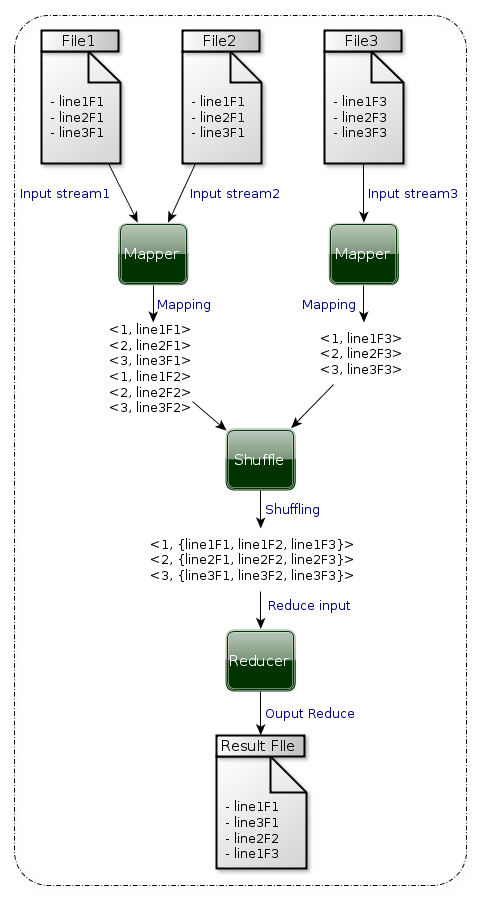
\includegraphics[width=280px,height=500px]{img/sampleProcess.png}
	\caption{Map and Reduce random sample process}\label{fig:sampleProcess}
\end{figure}

Now we present the algorithm with the behavior already shown is easier explained
the algorithm:

\begin{algorithm}
\begin{algorithmic}[1]
	\Require{$fileStream$ stream of file lines}
	\Statex
	\Function{Map}{$fileStream$}

		\State $lineNumber \leftarrow 1$
		\State $map<Integer, String> \leftarrow  \{\}$\\

		\ForEach{$line \in fileStream$} {

			\State $line \leftarrow getNextLineFromStream$

			\State $map.put$($lineNumber$, $line$)

		}

	\EndFunction
\end{algorithmic}
\end{algorithm}
